\chapter{Experiments and Evaluations}
\label{chapter:experiments_and_evaluations}
For the following tests, the second computational configuration of one NVIDIA TITAN X GPU
was used.  Only for the multiple device execution section was the first configuration implemented.
\section{Software Usage}
Besides the NVIDIA CUDA ecosystem, peripheral tools are offered to allow developers
to analyze program performance, and automatically recommend tips to increase performance.
Two such programs are \textit{nvprof}, a profiling tool comparable to gprof, and
\textit{nvvp}, a visual profiler for \Gls{CUDA} software. Both tools allow developers
to discover hot spots in their programs, optimize occupancy, the amount of registers
in use on an SM, and improve data transfer strategies.  For \Gls{RWoS}, occupancy
and computational intensity were both points of great interest. Since \Gls{RWoS}
is computer bound, rather than memory bound, the goal of this work was to continually
analyze and improve compute performance.  Data transfer optimization becomes of interest
when the dimensions and number of paths become so large, that intermediate results,
can no longer be stored on the device.  In this case a stream pipeline of concurrent
data transfer of intermediate results to the host, and computation would be of great
importance.  For this proof of concept implementation, the number of paths, and dimensions
are still low enough that pipelining was not yet necessary.  Nevertheless, \textit{nvvp}
was used to analyze the computational intensity of \Gls{RWoS} for \Glspl{GPU}.
\section{Profiling}
When profiling the code, it became apparent that since the code scales with the problem
size, i.e. dimension and number of path iterations, so to does the efficiency.  Occupancy,
describes the percentage of the number of CUDA cores on an individual SM filled
by the execution of a kernel.  This
percentage is therefore dependent on the number of CUDA cores available in the hardware at hand,
and the allocated number of threads per Block.
Due to the tread allocation strategy described in \ref{localRed}, occupancy was $50\%$
for dimensions bellow 32 and $93.9\%$ for dimension=64 due to the 64 CUDA cores
per SM in the TITAN X (see: \ref{hardwareTable}). For thread allocations greater than
64, occupancy remains at around $100\%$ threads are processed warp-wise, and 2 warps can
fit on one SM. Due to the near constant computational dead-time required for memory transfer time,
greater computational intensity can be achieved with higher dimensions or path iteration values.
\par
When profiling with \textit{nvvp} it was also reviled that the current implementation,
profiled with $dimension=64, iterations=10^{6}$, displayed a relatively low warp
execution efficiency of $56.2\%$.  This was due to a large number of predicated
instructions necessary to the computation.  According to \textit{nvvp}, if one
neglects the predicated instructions, the execution efficiency would be $100\%$.
Improving the warp efficiency would be a great starting point for future work.

\section{Execution on Multiple Devices}
To increase the performance of \Gls{RWoS} for \Glspl{GPU}, a multi-device implementation
was tested.  The goal was to gain a speed-up of 2 when running the code on two devices
simultaneously.  In order to divide the workload to two devices, the total number
of path iterations desired was divided by the number of devices available. Since,
result precision depends on the order of the number of iterations, is not dependent
on the exact number of iterations, the the total divided using integer devision,
and rounded to the nearest natural number for the sake of simplicity.  The two
devices selected, were GTX 560Ti. As mentioned in \ref{devicePar}, the code
was run simultaneously on both devices via CUDA streams, and the results were reduced
on the host, as before. To to space constrained on the motherboard, a PCIe-extender
ribbon cable was used to conned the second device to the motherboard. Initial tests
showed that for our test case (Dimension=512, Paths=65335) the running time dropped from
30.7 seconds for a single device, to 17,9 seconds when running on two devices,
resulting in a speed up of: $$ speedup = \frac{31.7 sec}{17.2 sec} = 1.84.$$ Unfortunately,
due to hardware failure (the PCIe extender cable was not very robust), further testing
of multiple device execution was not possible.  Never the less, the resulting code
is able to run on multiple devices, and will automatically run on all devices connected
to the host.

\subsection{Steps per Path}
one feature of the \Gls{RWoS} for \Glspl{GPU} is the ability to track the number of
steps per path.  This feature was added in order to verify theoretic values from \cite{Bornemann,DeLaurentis} and
\ref{epsilonComplexity}.  Through the addition of the runtime command line parameter
$-p$, the program returns the average number of steps per path.  By adding the $-l$
or $ \textendash log$
parameter, this value, along with other data o f interest will be saved to a local
.csv file.  As can be taken from the plot below, the number of steps increases
logarithmically over the number number of dimensions.  This is consistent with \cite{Bornemann, DeLaurentis}.
\begin{figure}
\begin{center}
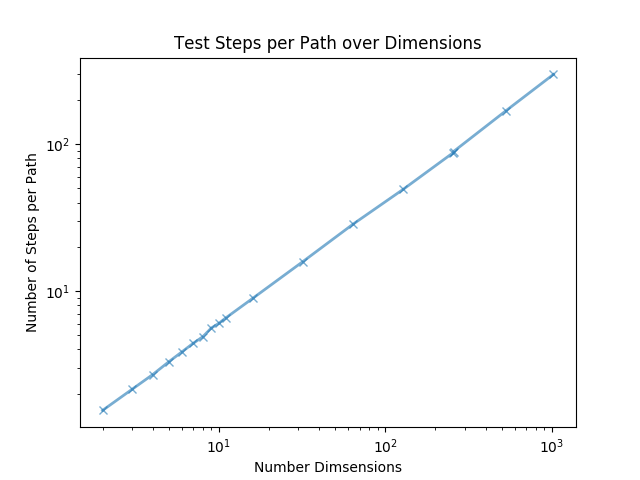
\includegraphics[width=10.0cm]{styles/pathsPerDim} \label{plot:pathsPerDim}
  \caption{Average number of steps per path sampled over a number of dimension}
\end{center}
\end{figure}
The linear regression of the above plot has a function of $$f(dimension)= 4.8108001661116715 + 0.2953577483675905*dimension.$$
A further point of interest, is weather the number of steps per path remains smaller
than the period of the random number generator, namely $2^{190}$ or $~1.5 * 10^{57}$.
Each thread has its own seed, therefore the number of random numbers generated per
thread is of interest.  This number is equal to
$$maxRand = total Paths \% 65535 * f(dimension)$$ and is constrained by
$$ maxRand \overset{!}{<} 2^{190}$$
%TODO: table for f dimension.

%TODO: use largest possible value and find maximum

\section{Accuracy and Error}
In order to test the convergence and accuracy of this \Gls{RWoS} on \Glspl{GPU} implementation,
the exact solution for a two dimensional case was attained via a Fourie series in
two dimensions \cite{Bornemann}.  The resulting value is  $$u(0,0) = 0.29468 54131 26055 26226$$.
This value will be used as a known solution in order to check accuracy and convergence.
The plot bellow shows the convergence of the two dimensional case.


\section{Scaling Tests}
As with many programs, it was of interest to investigate the scaling properties of
of this \Gls{RWoS} program in respect to iterations and dimensions. From the theory,
we expect to see a scaling behavior that $\mathcal{O}( N\log(N))$ in nature.
%TODO: only power 2 dimensions
The hyper linear increase in running time is most likely due to the transition from
block based path iteration scaling to loop based iteration scaling once the maximum
number of blocks has been reached.  Since the block loops are executed in serial,
and dependencies limit the optimizations between loops.
\section{Speedup}
One of the main goals of this work, was to show the possibility to decrease computation
time of \Gls{RWoS} by running the algorithm on \Glspl{GPU}.  To show the resulting
speed increase, we will compare a CPU version of \Gls{RWoS} to the \Gls{GPU} version
created in the scope of this work.  Though such comparisons are sometimes frowned
upon, and called "misleading" due to the difference in underlying processor architecture,
the goal of this work was to show the computational acceleration, regardless of architecture.
The examples provided below represents an arbitrary sample, but serves to show the
computational acceleration possible through \Glspl{GPU}.  As a base-line \Gls{CPU}
reference performance number, an implementation of \Gls{RWoS} in the language
Julia will be used.  Julia provides a high level interface to highly optimized
numerical programming.  The author also provides a version of \Gls{RWoS} written
in C++, but this version lacks numerical optimization and is therefore slower than
the Julia base line.  Therefore, the Julia version is used, in order to provide
the most conservative \Gls{speed-up} numbers possible.
\par
The data below goes to show that the super linear speed up of high dimensional
\Gls{RWoS} on \Glspl{GPU} confirms the presumption, that high dimensional problems
are well suited for \Glspl{GPU}.  Thanks to light context switches, large dimensional capabilities,
and the optimized \Gls{GPU} memory architecture and approach, the \Gls{GPU} implimentation
of \Gls{RWoS} performs very well.
